% THIS IS SIGPROC-SP.TEX - VERSION 3.1
% WORKS WITH V3.2SP OF ACM_PROC_ARTICLE-SP.CLS
% APRIL 2009
%
% It is an example file showing how to use the 'acm_proc_article-sp.cls' V3.2SP
% LaTeX2e document class file for Conference Proceedings submissions.
% ----------------------------------------------------------------------------------------------------------------
% This .tex file (and associated .cls V3.2SP) *DOES NOT* produce:
%       1) The Permission Statement
%       2) The Conference (location) Info information
%       3) The Copyright Line with ACM data
%       4) Page numbering
% ---------------------------------------------------------------------------------------------------------------
% It is an example which *does* use the .bib file (from which the .bbl file
% is produced).
% REMEMBER HOWEVER: After having produced the .bbl file,
% and prior to final submission,
% you need to 'insert'  your .bbl file into your source .tex file so as to provide
% ONE 'self-contained' source file.
%
% Questions regarding SIGS should be sent to
% Adrienne Griscti ---> griscti@acm.org
%
% Questions/suggestions regarding the guidelines, .tex and .cls files, etc. to
% Gerald Murray ---> murray@hq.acm.org
%
% For tracking purposes - this is V3.1SP - APRIL 2009

\documentclass{acm_proc_article-sp}
%\usepackage{[utf8x][inputenc]}
\usepackage[french,english]{babel}
\usepackage[utf8]{inputenc}
\usepackage{graphicx,url}
\newcommand{\subparagraph}{}
%\AtBeginDocument{\renewcommand{\abstract}{Resumé}}
\usepackage{titlesec}
\setcounter{secnumdepth}{4}


\titleformat{\paragraph}
{\normalfont\normalsize\bfseries}{\theparagraph}{1em}{}
\titlespacing*{\paragraph}
{0pt}{3.25ex plus 1ex minus .2ex}{1.5ex plus .2ex}
\begin{document}

\title{An Extendable Python Library To Manipulate Sensors Coupled To The Raspberry Pi}
%\subtitle{[Extended Abstract]
%\titlenote{A full version of this paper is available as
%\textit{Author's Guide to Preparing ACM SIG Proceedings Using
%\LaTeX$2_\epsilon$\ and BibTeX} at
%\texttt{www.acm.org/eaddress.htm}}}
%
% You need the command \numberofauthors to handle the 'placement
% and alignment' of the authors beneath the title.
%
% For aesthetic reasons, we recommend 'three authors at a time'
% i.e. three 'name/affiliation blocks' be placed beneath the title.
%
% NOTE: You are NOT restricted in how many 'rows' of
% "name/affiliations" may appear. We just ask that you restrict
% the number of 'columns' to three.
%
% Because of the available 'opening page real-estate'
% we ask you to refrain from putting more than six authors
% (two rows with three columns) beneath the article title.
% More than six makes the first-page appear very cluttered indeed.
%
% Use the \alignauthor commands to handle the names
% and affiliations for an 'aesthetic maximum' of six authors.
% Add names, affiliations, addresses for
% the seventh etc. author(s) as the argument for the
% \additionalauthors command.
% These 'additional authors' will be output/set for you
% without further effort on your part as the last section in
% the body of your article BEFORE References or any Appendices.

\numberofauthors{2} %  in this sample file, there are a *total*
% of EIGHT authors. SIX appear on the 'first-page' (for formatting
% reasons) and the remaining two appear in the \additionalauthors section.
%
\author{
% You can go ahead and credit any number of authors here,
% e.g. one 'row of three' or two rows (consisting of one row of three
% and a second row of one, two or three).
%
% The command \alignauthor (no curly braces needed) should
% precede each author name, affiliation/snail-mail address and
% e-mail address. Additionally, tag each line of
% affiliation/address with \affaddr, and tag the
% e-mail address with \email.
%
% 1st. author
\alignauthor
Edivaldo M. F. de Jesus Jr\titlenote{Aluno do curso de An\'alise e Desenvolvimento de Sistemas(ADS)}\\
       \affaddr{Instituto Federal da Bahia}\\
       \affaddr{Rua Em\'idio dos Santos, S/N}\\
       \affaddr{Barbalho, Salvador Bahia}\\
       \email{juniorug@gmail.com}
% 2nd. author
\alignauthor
Manoel C. M. Neto\titlenote{Doutor em Ci\^encia da Computa\c{c}\~ao e Professor do Curso de An\'alise e Desenvolvimento de Sistemas}\\
       \affaddr{Instituto Federal da Bahia}\\
       \affaddr{Rua Em\'idio dos Santos, S/N}\\
       \affaddr{Barbalho, Salvador Bahia}\\
       \email{manoelnetom@ifba.edu.br}
}
% There's nothing stopping you putting the seventh, eighth, etc.
% author on the opening page (as the 'third row') but we ask,
% for aesthetic reasons that you place these 'additional authors'
% in the \additional authors block, viz.

\date{13 April 2015}
% Just remember to make sure that the TOTAL number of authors
% is the number that will appear on the first page PLUS the
% number that will appear in the \additionalauthors section.

\maketitle
\selectlanguage{french} 
\def\startRÉSUMÉ{}

\begin{abstract}

La convergence des technologies de radio, microprocesseurs et appareils numériques personnels conduit à la notion de l'informatique ubiquitaire où les dispositifs intelligents, mobiles et fixes, de coordonner les uns avec les autres pour fournir aux utilisateurs un accès immédiat et universel aux nouveaux services de manière transparente, visant à accroître humaine capacités. Ce travail vise à définir, mettre en œuvre et valider la conception et la mise en œuvre d'une bibliothèque Python extensible pour manipuler des capteurs / actionneurs couplés à la Raspberry Pi en utilisant le module de framboise-GPIO-python. La bibliothèque utilise le modèle de fabrique abstraite pour se assurer que les capteurs / actionneurs et les événements de la même famille étant utilisés en conjonction avec moyen garanti. Sur les autres plateformes, comme Arduino, les API fournissent bibliothèques qui encapsulent la complexité de mise en œuvre et ne offrent que l'interface à utiliser. Ces bibliothèques ne existent pas encore officiellement pour ceux qui veulent utiliser Pyton comme langage de développement appliqué à la Raspberry Pi. Cet article encourage l'utilisation des technologies open source, en raison de la croissance de la libre circulation du matériel, la déduction de la possibilité d'une alternative pour les ingénieurs et les professionnels à développer leurs projets et fournir à la diffusion des connaissances. Le projet présente également les résultats obtenus en utilisant certains des capteurs mis en œuvre, la modélisation du système et les résultats décrits et 






%A converg\^encia das tecnologias de r\'adio, dos microprocessadores e dos dispositivos eletr\^onicos digitais pessoais est\'a levando ao conceito de Computa\c{c}\~ao Ub\'iqua no qual dispositivos inteligentes, m\'oveis e estacion\'arios, coordenam-se entre si para prover aos usu\'arios acesso imediato e universal a novos servi\c{c}os, de forma transparente, que visam aumentar as capacidades humanas. Este trabalho  tem como objetivo definir, implementar e validar o projeto e implementa\c{c}\~ao de uma biblioteca Python extens\'ivel para manipular sensores / atuadores acoplados ao Raspberry Pi usando o m\'odulo raspberry-gpio-python. A biblioteca utiliza o Padr\~ao Abstract Factory para garantir que sensores/atuadores e eventos de mesma fam\'ilia sejam usados em conjunto de forma garantida. Em outras plataformas, como no Arduino, as APIs oferecem bibliotecas que encapsulam a complexidade de implementa\c{c}\~ao e oferecem apenas a interface para o uso. Essas bibliotecas ainda n\~ao existem formalmente para quem quer usar Pyton como linguagem de desenvolvimento aplicada ao Raspberry Pi. Este artigo incentiva o uso de tecnologias de c\'odigo aberto, devido ao crescimento da livre circula\c{c}\~ao de hardware, inferindo a possibilidade de uma alternativa para engenheiros e profissionais para desenvolver seus projetos e fornecem a dissemina\c{c}\~ao do conhecimento. O projeto apresenta tamb\'em os resultados obtidos utilizando alguns dos sensores implementados, a modelagem do sistema e os resultados obtidos descritos e analisados.

%This paper provides a sample of a \LaTeX\ document which conforms to
%the formatting guidelines for ACM SIG Proceedings.
%It complements the document \textit{Author's Guide to Preparing
%ACM SIG Proceedings Using \LaTeX$2_\epsilon$\ and Bib\TeX}. This
%source file has been written with the intention of being
%compiled under \LaTeX$2_\epsilon$\ and BibTeX.

%The developers have tried to include every imaginable sort
%of ``bells and whistles", such as a subtitle, footnotes on
%title, subtitle and authors, as well as in the text, and
%every optional component (e.g. Acknowledgments, Additional
%Authors, Appendices), not to mention examples of
%equations, theorems, tables and figures.

%To make best use of this sample document, run it through \LaTeX\
%5and BibTeX, and compare this source code with the printed
%output produced by the dvi file.

\end{abstract}

\selectlanguage{english} 
\keywords{Ubiquitous Computing,Internet of Things, Raspberry Pi, Sensor, Python} % NOT required for Proceedings


\section{Introduction}

The UbiComp in its various ramifications and applications, is considered by many as the twenty-first century's new paradigm of computing. It is the area of computing that studies the coupling of the physical world to the world of information and provides an abundance of services and applications, allowing users, machines, data and objects of physical space interact with each other seamlessly. The theme is considered one of the great challenges of research in Computer Science by the National Science Foundation (NSF) [1] and is also present in Computing search Grand Challenges report in Brazil from 2006 to 2016 [2], published by the Brazilian Computer Society (SBC).
\newline
\newline
Researches on ubiquitous computing are being held on topics such as: basic access to any wireless device, mobility support within the network transparently, safety, context treatment, efficient use of energy, presentation of multimedia content and so on. This work is focused on building intelligent interactive environments. In these environments, the fundamental idea is to create ways to avoid that the user needs to go to the computer/device, allowing many of these working at a distance. The use of platforms to integrate the devices that make up these environments is one of the key points to create it. Currently there are some options to fill this gap. This text emphasizes one: the project Raspberry Pi [3,4].
\newline
\newline
Raspberry Pi is a widely used platform for professionals who are interested in the field of ubiquitous applications. It provides basic interfaces for creating small projects and / or for those who must be fed by battery. The platform allows you to use high-level programming languages that are quite widespread as C / C ++, Python and Java. The Raspberry allows the development of a range of projects. For example, home automation (turn on and off electrical devices, remote control for TV, Air-conditioners, etc.), eBook and Audiobook readers and so on.
\newline
\newline
If we seek a way to access the Raspberry Pi bus we shall find a lot of papers in Python. Which incidentally, brings the acronym of the device name (Pi from Python). However, we cannot find any library that abstracts the details of wiring a sensor or actuator to the Raspberry allowing the user takes care just in read the data already processed and/or converted.
\newline
\newline
The developer must have a degree of experience that can be considered basic to a computer professional, but advanced for those who are not.
\newline This paper is structured as follow:
\begin{itemize}
\item Section 2 present several technologies involved in the preparation of this monograph, aimed to introduce important concepts of Computer area in which the context of the project is inserted
\item Section 3 shows correlated works
\item Section 4 presents the details of the executed implementation
\item Sections 5 and 6 address the testing methodologies used and the results obtained during system validation. 
\item The last section presents the conclusions.
\end{itemize}

\section{THEORETICAL BACKGROUND}

\subsection{General Context}

The term Ubiquitous Computing was first defined by Mark Weiser [33] in the late 80. At this time, Weiser predicted an increasing in functionality and availability of computing services to end users and, on the other hand, he predicted a decreased visibility of these services. For Weiser, the computing would not be exclusive of a computer. He believed that in the future there would be several different devices connected to each other. At a time when users were using PCs (desktops) and that knowledge needed to operate a computer,  Weiser bet on a future where the focus of the users would be the task itself, and not the tool used. In this way, they would use the computer without realizing or require specific technical knowledge. [34]
\begin{figure}[h]
    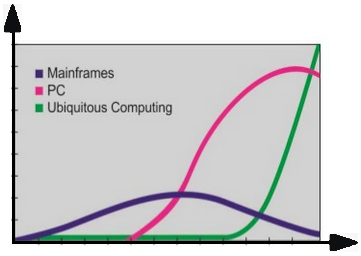
\includegraphics[width=0.4\textwidth,natwidth=610,natheight=642]{pictures/era.png}
    \caption{Ages of Computing}
\end{figure}
\newline
\newline
The passage of time has shown that betting Weiser was right. For Weiser, [35] evolution of computing has gone through two ages to reach to ubiquitous computing. The first was called the age of mainframe, where many people shared the same computer. The second era was the PC, where each computer was used by one person. Currently, the evolution of distributed information systems, the network connections type options'  expansion, mobile computing and the various types of applications on non-conventional computing devices, are just some of the examples that can confirm: the Ubiquitous Computing (the third age) is already a reality.
\newline
\newline


Terms such as ubiquitous computing, pervasive computing, nomadic computing, invisible computing, mobile computing and many others, have been used often interchangeably, although they differ conceptually and employing different organization of ideas and management of computer services. Insofar as each area progresses, these concepts will be better understood and its definitions will become clearer. This section presents the key concepts needed to understand the UbiComp besides presenting some project examples in the literature.

\subsection{Mobile Computing}

Mobile computing is based on the ability of a user to load or move (physically) computer services wherever it moves. In this context, the computer becomes an ever-present device that expands the ability of a user to use the services it offers, regardless of their location. Combined with the ability to access the network, mobile computing has transformed the computing an activity that can be taken almost anywhere.
\newline
\newline
An important conceptual limitation of mobile computing is that the computational model used in most applications does not change while users are moving. It means that a device is not able to obtain information on the physical context in which computation occurs, and consequently also can not adapt to the new context correctly. A solution to accommodate the changing context would pass to users the responsibility to monitor and manually configure an application / device to the extent that it moves. However, this solution is not well accepted by most users. This limitation was one of the inspirations for pervasive computing .

\subsection{Pervasive Computing}

The concept of pervasive computing implies that the computer is embedded invisibly in the environment to the user [24]. In this conception, the computer has the ability to: i) obtain environmental information in which it is embedded and ii) use it to build dynamically computational models that allow you to control, configure and tune the application to better suit the needs of a device or user. For this to be possible, the key point is the ability of computers be able to act as "smart" in the environment where users move. This environment is usually populated by computational sensors and services.

\subsection{Ubiquitous Computing}

As can be seen in Figure 1.1, the UbiComp can be defined as a computer area positioned between the Mobile Computing and Pervasive Computing [14, 24]. Ubiquitous is an adjective originated from Latin (ubiquu) which means "that is at the same time everywhere". Ubiquitous computing benefits from the advances in mobile and pervasive computing and arises from the need to integrate mobility with the functionality of pervasive computing. The term ubiquitous computing will be used here as a junction of pervasive computing and mobile computing. The justification to perform a distinction of these terms is a device that is embedded in an environment, not necessarily is mobile.
\begin{figure}[h]
    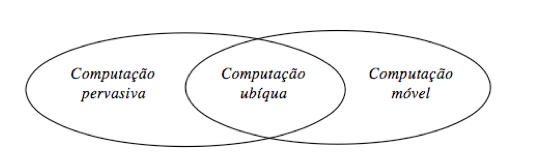
\includegraphics[width=0.4\textwidth,natwidth=610,natheight=642]{pictures/ubiq.png}
    \caption{Ubiquitous Computing: intersection between pervasive and mobile computing}
\end{figure}
\newline
\newline
Research in Ubiquitous Computing approach about the technologies and infrastructure that enable the deployment of ubiquitous applications through a number of issues including the following:

\begin{itemize}
\item how to design hardware and operating systems for sensor platforms?
\item how to allow devices to find each other and to use your services?
\item how to allow systems involving limited processing resources and energy, to work well?
\end{itemize}

Generally, ubiquitous applications receive sensor data from other service providers devices, manage user actions, provide support mobility and use context information to perform tasks [6]. A ubiquitous system itself has a set of requirements, peculiarities and challenges that influence the design, implementation, deployment and evaluation of its project. [24] These are cornerstones of UbiComp and quite different from those used in the development of systems for PC’s. Among these points, we can cite as an example.:

\begin{enumerate}
\item Resource-Constrained Devices; 	
\item Volatile Execution Environments; 	
\item Heterogeneous Execution Environments;
\item Fluctuating Usage Environments;
\item Invisible Computing;
\item Security and Privacy;
\end{enumerate}


\subsection{Internet of Things}

The Internet of Things (IoT) is a multidisciplinary field, covering a wide range of subjects, from purely technical issues (eg, routing protocols, semantic queries) to a mixture of technical and social problems (security, privacy, usability) as well as social and business topics. The existing internet of things’ applications are potentially diverse. Monitoring of environmental and personal health, monitoring and control of industrial processes, including agriculture, smart spaces and smart cities are just some examples of the IoT applications [5].

\subsection{Hardware}

One of the fundamental requirements for developing ubiquitous systems is the use of hardware such as sensors, microcontrollers, communication devices (network cards, Bluetooth, etc.) and storage, among others. For example, sensors allow transform use of interactive environments from more transparent interfaces. Currently, there are some platforms that allow insert and control various types of sensors, using of communication interfaces and storage units. This section presents and details the main hardware devices available for the development of ubiquitous systems.


\subsubsection{Sensors and Actuators}

Sensors are devices that allow us to capture information from the environment in which they are inserted, such as temperature, pressure, presence, humidity, smoke detector, light intensity, among others. In general, the sensors work transforming parts of a physical quantity into an electrical signal, which in turn can be interpreted by electronic devices [7]. In other words, sensors are components that allow an electronic device to interact with the real world.
\newline
\newline
According to [7], when the sensors operate directly, transforming one form of energy into another are called transducers. The sensors where operations occur indirectly alter their properties, such as resistance, capacitance or inductance, under the action of physical grandeur so that this change is roughly proportional. For example, the light sensor LDR (Light-dependent resistors) vary inversely its resistance the amount of light falling on it. Thus, when there is a large amount of light falling on the sensor, they have a very low resistance and this allows the flow of electric current increases, whereas when there is little light, they have a high resistance and prevent current flow.
\newline
\newline
An actuator as well as a sensor is a transducer that converts one form of energy into another, and can also do the opposite [7]. In other words, rather than just  transform parts of a physical quantity into an electrical signal, it can transform an electrical signal into a physical quantity such as motion, magnetism, heat, among others. For example, the relays are electromechanical devices that work with small power, but are able to control external circuits that involve high currents. They are basically composed of a coil and a set of contacts. When a current flows through the coil it creates a magnetic field that attracts and closes the contacts, remaining as long as power supply in the coil. As a result, it allows the passage of energy through the relay.

\subsubsection{Arduino}

Arduino was created in 2005 by Massimo Banzi and David Mellis in Italy with the goal of use as an electronic learning tool and programming for design students, so that they would use in art projects, interactivity and robotics. Electronic learning was expensive: a microcontroller was costing 100 euros. So they decided to make their own board. Sought employees and thus created an efficient technology, accessible and compatible with Windows, Mac and Linux.
\newline
\newline
Arduino is a platform that popularizes the concept of free hardware. In the book Getting Started with Arduino, Massimo Banzi describes the Arduino as a physical open-source computing platform based on a simple board with input/output pins that implements the Processing language. It is a small but powerful board constituted by a microcontroller that can be easily programmed via a Universal Serial Bus interface (USB) and able to build electronic devices and interesting systems.
\newline
\newline
Working with the construction of a hardware requires much time and effort, because is necessary to create new circuits, use various components such as resistors and capacitors and many welds. Using Arduino board abstracts much of this construction process, making it simpler, allowing people from different fields of knowledge being able to build their projects. The platform is widely used worldwide for offering advantages such as:


\begin{itemize}
\item A multiplatform environment that can run all major operating systems such as Windows, Linux and MacOS.
\item Is an open-source hardware, ie, the circuit design is available so that if someone is interested in creating your own card, just buy the necessary components.		
\item Hardware cost is low.					
\item Is possible program it via a USB cable instead of a serial port. Remember that today's computers do not have serial ports.	
\item It has a development environment with intuitive interface for easy use.
\end{itemize}

The fact that both the hardware and the Arduino software be developed in an open, patent-free, allows its projects to be recreated in different ways. The adoption of open hardware concept motivates those who create projects to contribute with functions and libraries for the Arduino. Is knowledge about knowledge, the same principle of free software.
\newline
\newline
Note that there is not necessary advanced knowledge in electronics to use the platform. But for those who are interested in deepening the knowledge in this area, there are several available materials that can help, for example, in [19].

\paragraph{Features}

There are dozens of Arduino’s types with different sizes, amount of memory and interfaces. To illustrate the possibilities of use and describe the Arduino, we will use the model "UNO" as an example.
\newline
\newline
The hardware Arduino UNO can be sub-divided into six blocks described below. They can be seen in Figure XXX.
\newline
\newline
Power Supply: Responsible for receiving the external power supply, which can have a voltage of at least 7 Volts, 35 Volts as the maximum and a minimum current of 300mA. The power supply filter and then regulates the input voltage for two outputs of 5 and 3.3 volts each. The function of this block is to deliver the voltages of 5 and 3.3 Volts for that the Central Processing Unit (CPU) and other circuits work.
\newline
\newline
CPU Core: The core processing of an Arduino board is a microcontroller chip (see section 2.2.1). Arduino developers have chosen to use the company's microcontroller line of ATMEL4 company. The line used is the ATmega. There are official Arduino boards with several models in this line, but the most common are the boards with ATmega8 chips, AT-Mega162 and ATMEGA328P. These models differ in the amount of Read Only Memory (ROM) and configuration of input and output modules available.
\newline
\newline
Inputs and Outputs: The number and options of input and output from an Arduino microcontroller depend on the chip used. The ATmega8, for example, has 28-pin electrical connectors. Is through these pins that you can control the chip, send data to your memory and trigger external devices connected to the Arduino. The pins are divided into:

\begin{itemize}
\item Digital pin to input or output (programmable) - 14 pins;	
\item Analog input pins or digital input / output (programmable) - 6 pins;
\item Power pins (gnd, 5V, 3.3V) - 5 pins;
\item Reset pin - 1 pin;	
\item Pins to connect the crystal oscillator - 2 pins;
\end{itemize}

The first two items on the list are the useful pins. They are the ones that are available for a programmer use. Is through these pins that the Arduino is coupled to the sensors to capture environmental information. Among the 14 digital input / output pins there are 2 pins that match the serial communication module USART (Universal Synchronous Asynchronous Receiver Transmitter) [13]. This module allows communication between a computer (for example) and the Arduino (see Special Pins section). All pins (digital or analog) have more than one function. The pins can be input or output, some may serve for analog readings and also for digital input. The roles of each are defined in the code of possible programs that can be run on the Arduino.

\paragraph{Digital Inputs}

There are 20 pins that can be used as digital inputs. There are 14 digital pins and more 6 analog pins. When a pin is programmed to function as digital input, you use a command that, when executed, performs the "reading" of the voltage applied to it. Then, after running this command, you can know if the pin is in a "high" or "low" state (on or off). 
\newline
\newline
From the electrical point of view, the program can tell if a pin is fed with 0 (zero) or 5 Volts. This function is usually used to identify whether a button is pressed or a sensor is capturing some environmental information. Note that the digital input function delivers only the values 0 or 1 (no voltage or with voltage). You can not know how much voltage is being applied to the pin. For this you must use the analog inputs.

\paragraph{Analog Inputs}

There are 6 analog inputs. Unlike a digital input, which only informs whether there is or not a voltage applied to its pin, the analog input is capable of measuring the applied voltage. Through analog input, you can use sensors that convert any physical quantity in a voltage value which is then read by the analog input.

\paragraph{Digital outputs}

With a digital output is possible only two types of values (0 or 5 volts, 1 or 0, etc.). From a pin programmed as digital output is possible for example light up an LED, connecting a relay, trigger a motor, etc. You can program the Arduino (UNO) for at most 20 digital outputs. But you can use one or more pins to control a pack of other pins and this can increase this limit use of digital pins.

\paragraph{Special Pins}

Arduino pins have some special characteristics which can be used from the software functions encoded by a software programmer. Are they:
\begin{itemize}

\item PWM - Pulse Width Modulation [4]: Treated as analog output, it is actually a digital output that generates an alternating signal (between 0 and 1) where the time that the pin is in level 1 (on) is controlled. It is used, for example, for engine speed control, or generate voltages with values controlled by the program. For the PWM communication may use pins 3, 5, 6, 9, 10 and 11. The PWM function is detailed in Section 3.2.1;

\item USART - Universal Serial asynchronous receiver/transmitter: One pin can be used to transmit and another to receive data in serial asynchronous format. For example, you can connect a data transmission module via bluetooth and allow communication with the Arduino remotely. Are reserved for USART pins 0 (RX receives data) and 1 (tx sends data);

\item Analog Comparator: These pins can be used to compare two external voltages without making a program that reads these tensions and compare. This is a very quick way to compare voltages and is made by the hardware without involving programming. Are used pins 6 and 7;
\item External Interrupt: The pins 2 and 3 can be programmed to notify the software running on the Arduino about any change in its state. For example, you can connect a button to these pins and every time someone presses the button the program is diverted to a particular block set by the programmer.

\item SPI Port - Serial Peripheral Interface [29]: These are pins that allow synchronous serial communication faster than USART. They allow for example to connect memory cards (SD) and many other things. Are used for this purpose the pins 10 (SS), 11 (MOSI), 12 (MISO) and 13 (SCK).
\end{itemize}

\subsubsection{Raspberry Pi}

Raspberry Pi is a small computer, approximately with the size of a credit card. It can be used to do many things that are done by a common personal computer (RASPBERY PI FUNDATION, 2014a). In addition, it can also be used in electronic projects because it has a hardware interface: The general purpose input/output port (GPIO). The Raspberry Pi Foundation, creator of the project, is an educational charity headquartered in the UK and aims to help and encourage the teaching of computer science in schools.
\newline
\newline
This computer came up with the intention of reconnecting children and youth in computer programming and stimulate the creation of new projects so there is not only the consumption of the technology created by the market. While in the 1990s there was a growth in the number of children and youth who developed programming skills, starting in the 2000s, this number started to decline. (Raspbery PI Foundation, 2014b).
\newline
\newline
With the realization that, year by year, the students were moving away from programming and reducing the development of skills in computer science. The researchers Eben Upton, Rob Mullins, Jack Lang and Alan Mycrof, from the Computer Laboratory of University of Cambridge had the idea of creating a platform that would allow to reconcile the programming students  and handling computers. (DENNIS, 2013) From 2006 to 2008, early versions of what is now the Raspberry Pi was developed. From 2008, with the expansion and emphasis on mobile devices, the devices are becoming more efficient and cheaper which enabled the launch of the Raspberry Pi model B to the public in February 2012 for \$ 35.
\newline
\newline
The proposal of the Raspberry Pi is therefore be a low-cost computer, with the ability to interact with the outside world through the sensor coupling. As seen previously, it was thought to be used in the educational environment, in order to assist and encourage the teaching of programming and help understand the operation of computers. However, the Raspberry Pi has been used by people of all ages and interests in various projects, for example, projects involving automation, sensing and robotics, games, multimedia, networks and servers.
\newline
\newline
Currently there are three  Raspberry Pi models: The model A, which costs \$ 25 and the B and B+ models, which costs \$ 35. As for the price, there is not much difference between the hardware models. The main differences are the amount of USB ports (1, 2 and 4 in the models A, B and B +, respectively), the Ethernet port (model A does not have) and ram (256MB on the model A against 512 for the others).
\begin{figure}[h]
    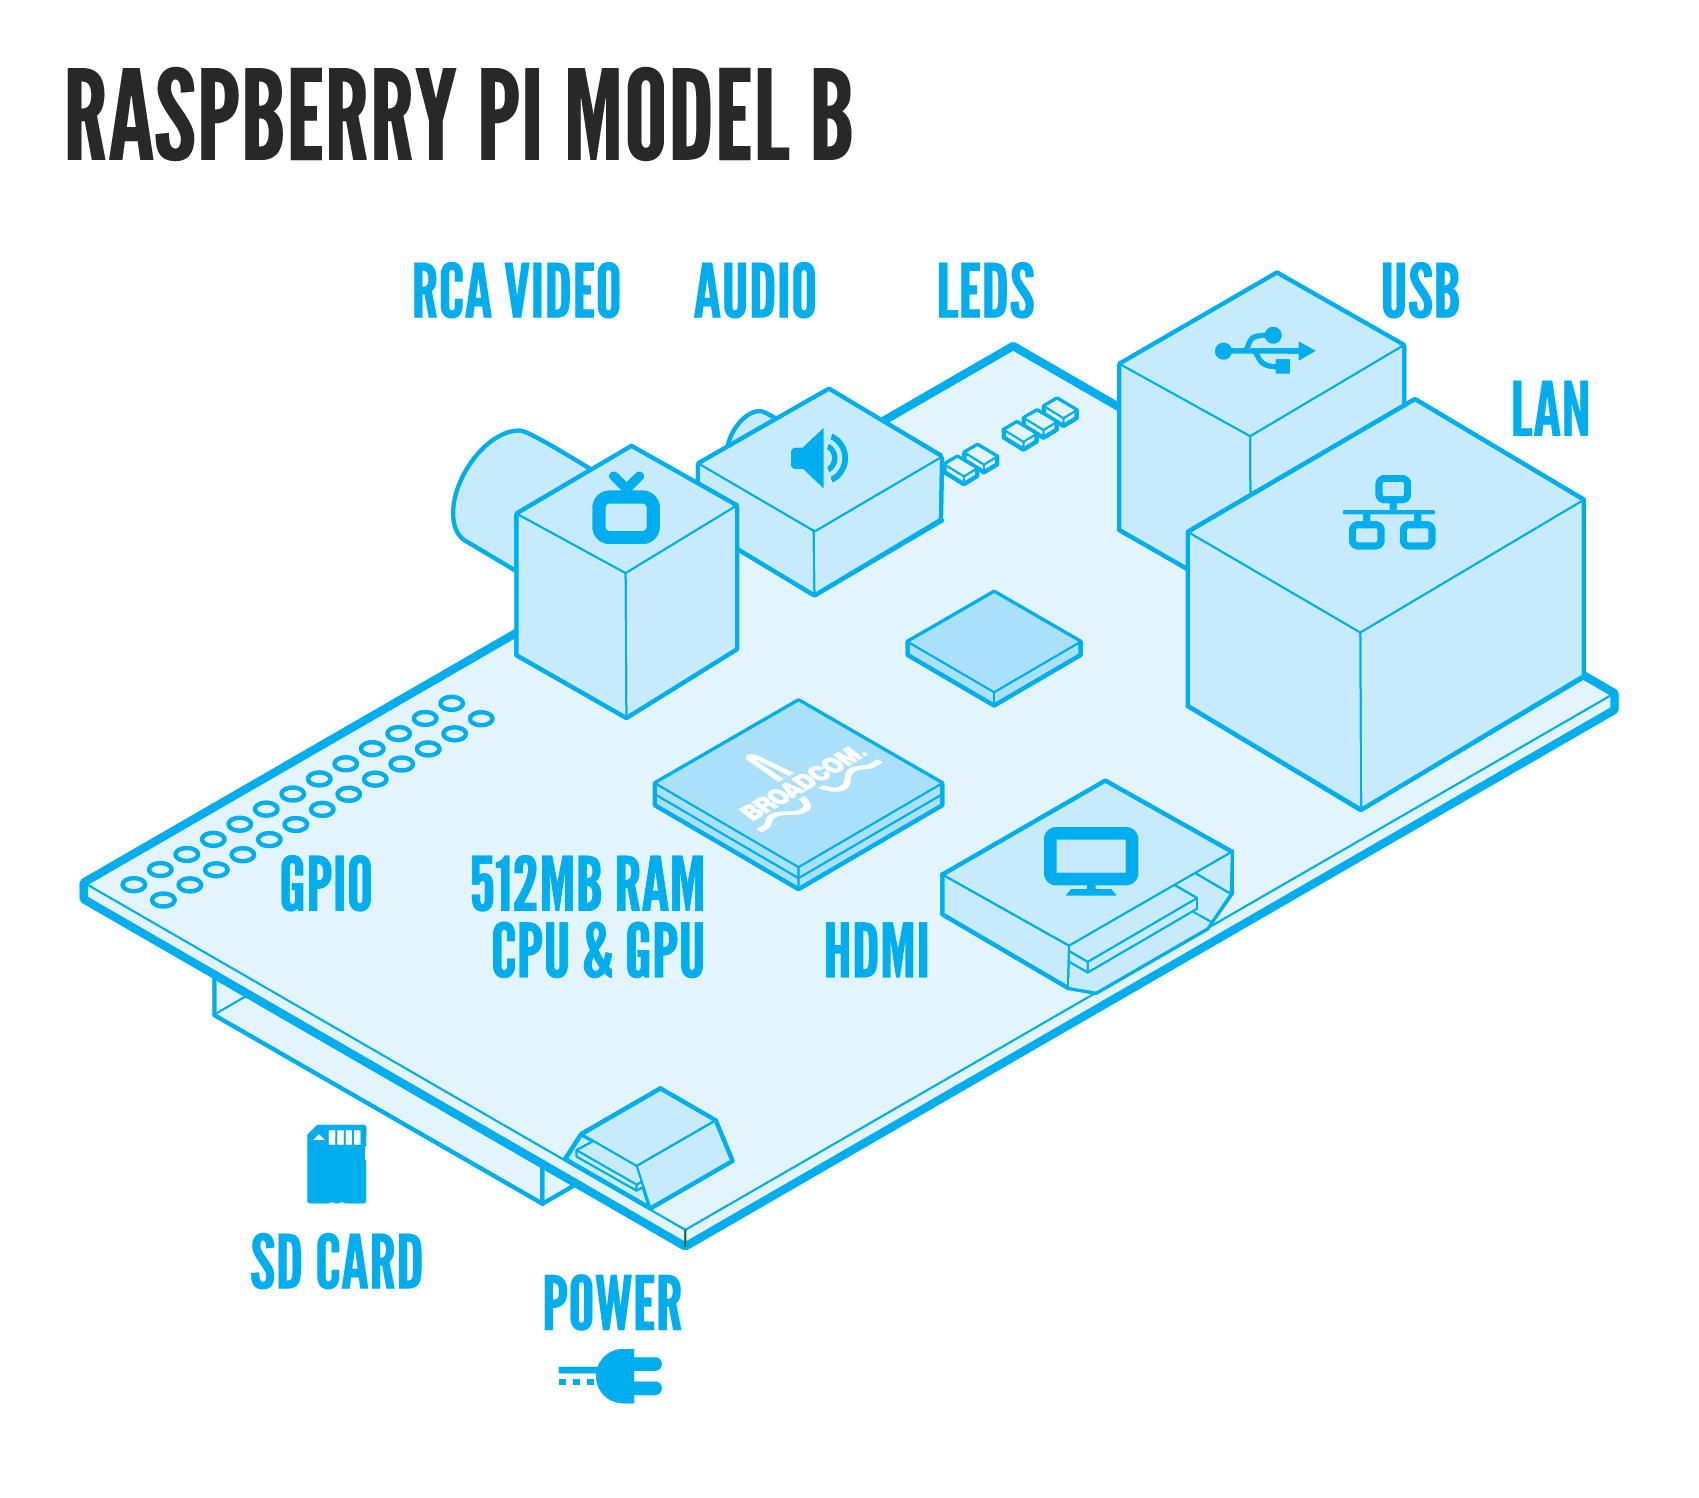
\includegraphics[width=0.5\textwidth,natwidth=610,natheight=642]{pictures/RaspiModelB.png}
    \caption{Raspberry Pi Components, model B. Font: (RASPBERY PI FUNDATION, 2014c)
}
\end{figure}

\paragraph{Special Pins}

\begin{itemize}
\item Display Serial Interface Connector (DSI)- This connector receives a flat-ribbon cable of 15 pins that can be used to communicate with an LCD or organic light-emitting diode (OLED) display screen.

\item Camera Serial Interface(CSI) Connector  - This port allows a camera module be directly coupled to the card.

\item P2 and P3 connectors - These two rows of connectors are JTAG connectors for test to Broadcom chip (P2) and LAN9512 network (P3). Due to the proprietary nature of Broadcom chipset, these connectors are unlikely to be of much used.

\item Power Pins - The header provides 5V on Pin 2 and 3.3V on Pin 1. The 3.3V supply is limited to 50mA. The 5V supply draws current directly from your microUSB supply so can use whatever is left over after the board has taken its share. A 1A power supply could supply up to 300mA once the board has drawn 700mA.

\item Pin Protection - Most of the pins in the header go directly to the Broadcom chip. It is important to carefully design the components you attach to them as there is a risk you will permanently damage your Pi. Short circuits and wiring mistakes could also ruin your day so double check everything. A multimeter is probably going to help a lot here as you can double check wiring before you connect to the Pi.
\item  Basic GPIO - The header provides 17 Pins that can be configured as inputs and outputs. By default they are all configured as inputs except GPIO 14 \& 15. In order to use these pins you must tell the system whether they are inputs or outputs. This can be achieved a number of ways and it depends on how you intend to control them. I intend on using Python.
\end{itemize}

\paragraph{GPIO in Python}

The easiest way to control the GPIO pins is using the RPi.GPIO Python library. Installing the library is easy if you follow my RPi.GPIO Installation Guide. Once installed using the pins is as easy as in figure 2:
\begin{figure}[h]
    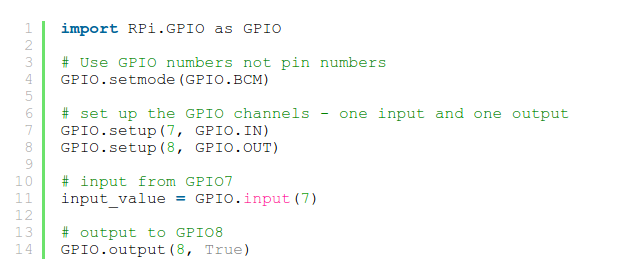
\includegraphics[width=0.57\textwidth,natwidth=610,natheight=642]{pictures/gpio.png}
    \caption{controlling gpio with Python}
\end{figure}

\paragraph{General Purpose Input/Output}

Another important aspect of hardware from Raspberry is the group of GPIO pins. These pins are programmable ports to input and output data used to provide an interface between the board and peripherals, microcontrollers/microprocessors, sensors, actuators, etc. The GPIO interface is fundamental for building intelligent interactive environments. It is the interface between the Raspberry and the real world. In simple terms, you can consider the GPIO pins as switches that can be turned on/off.
\newline
\newline
Similarly to the Arduino, besides the GPIO, the Raspberry also supports PWM, UART and SPI. Of the 26 pins available, 17 are reserved for GPIO and 8 are used for power and ground. Figure 2.6 shows the GPIO interface. The pins can be used via code written in a programming compatible language like Python, Scratch, Java, among others [8].
The GPIO pins are available on the PCB via a header and allow you to interface the Pi to the real world.

\paragraph{GPIO.BOARD and GPIO.BCM}

The GPIO.BOARD option specifies that you are referring to the pins by the number of the pin the the plug - i.e the numbers printed on the board (e.g. P1) and in the middle of the diagrams below.
\newline
\newline
The GPIO.BCM option means that you are referring to the pins by the "Broadcom SOC channel" number, these are the numbers after "GPIO" in the green rectangles around the outside of the below diagrams:
\newline
\newline
Unfortunately the BCM numbers changed between versions of the Model B, and you'll need to work out which one you have guide here. So it may be safer to use the BOARD numbers if you are going to use more than one pi in a project.

\paragraph{WiringPi}

WiringPi is a library for access to GPIO interface written in C. Its use can be performed with C, C ++, or other programming languages through wrappers (WIRING PI, 2014). Wrapper is an outer layer that extends WiringPi and can be implemented in different programming languages. This will allow the programmer to carry out projects not only in C or C ++, but also in language implemented by the wrapper. There are wrappers being developed in various languages such as Java, Ruby and Pyton. This last will be used in this paper from the wrapper raspberry-gpio-python.

\paragraph{raspberry-gpio-python}

\section{JUSTIFICATION}

As with other platforms, Raspberry Pi allows coupling several sensors whose handling can be made from raspberry-gpio-python or any other API available. On other platforms, such as the Arduino, the APIs provide libraries that encapsulate the complexity of implementation and offer only the interface to use. These libraries do not yet exist formally for those who want to use Python as a development language for Raspberry Pi.
\newline
\newline
This may be a consequence of run under the Linux kernel which is not suitable for real time applications - it is multitasking O/S and another process may be given priority over the CPU, causing jitter in the program[??].

\section{CORRELATED WORK}

\section{APPLICATION DEVELOPMENT}

\subsection{Method/Methodology}

\subsection{Functional Requirements}
 
\subsection{Non-functional Requirements}

\subsection{Why not use Java}

\subsection{Architecture}

\subsection{tests}


\section{CONCLUSIONS}


\section{FUTURE WORK}

\section{REFERENCES}
\subsection{Citations}

\subsection{Tables}






\subsection{Figures}



\subsection{Theorem-like Constructs}


%
% The following two commands are all you need in the
% initial runs of your .tex file to
% produce the bibliography for the citations in your paper.
\bibliographystyle{abbrv}
\bibliography{sigproc}  % sigproc.bib is the name of the Bibliography in this case
% You must have a proper ".bib" file
%  and remember to run:
% latex bibtex latex latex
% to resolve all references
%
% ACM needs 'a single self-contained file'!
%
%APPENDICES are optional
%\balancecolumns
\appendix
%Appendix A
\section{Headings in Appendices}
The rules about hierarchical headings discussed above for
the body of the article are different in the appendices.
In the \textbf{appendix} environment, the command
\textbf{section} is used to
indicate the start of each Appendix, with alphabetic order
designation (i.e. the first is A, the second B, etc.) and
a title (if you include one).  So, if you need
hierarchical structure
\textit{within} an Appendix, start with \textbf{subsection} as the
highest level. Here is an outline of the body of this
document in Appendix-appropriate form:
\subsection{Introduction}
\subsection{The Body of the Paper}
\subsubsection{Type Changes and  Special Characters}
\subsubsection{Math Equations}
\paragraph{Inline (In-text) Equations}
\paragraph{Display Equations}
\subsubsection{Citations}
\subsubsection{Tables}
\subsubsection{Figures}
\subsubsection{Theorem-like Constructs}
\subsubsection*{A Caveat for the \TeX\ Expert}
\subsection{Conclusions}
\subsection{Acknowledgments}
\subsection{Additional Authors}
This section is inserted by \LaTeX; you do not insert it.
You just add the names and information in the
\texttt{{\char'134}additionalauthors} command at the start
of the document.
\subsection{References}
Generated by bibtex from your ~.bib file.  Run latex,
then bibtex, then latex twice (to resolve references)
to create the ~.bbl file.  Insert that ~.bbl file into
the .tex source file and comment out
the command \texttt{{\char'134}thebibliography}.
% This next section command marks the start of
% Appendix B, and does not continue the present hierarchy
\section{More Help for the Hardy}
The acm\_proc\_article-sp document class file itself is chock-full of succinct
and helpful comments.  If you consider yourself a moderately
experienced to expert user of \LaTeX, you may find reading
it useful but please remember not to change it.
\balancecolumns
% That's all folks!
\end{document}
